\section{Forward and backward propagation}

  There are two main differences between the forward and backward pass
  computation.  While the forward pass computes convolutions, the
  backward pass computes cross--correlations.  Performing a
  cross--correlation is equivalent to performing a convolution with
  kernel that is reflected along all dimensions.  Secondly, during the
  forward pass the convolution is performed only for locations where
  the kernel is fully contained inside the image\footnote{This is
    known as a \texttt{valid} convolution in MATLAB.}.  Thus, the
  output image has dimensions smaller or equal to the input image.  In
  the backward pass, \texttt{full} convolution/cross--correlation is
  performed.  Image size increases because an output voxel exists
  whenever the sliding window has some overlap with the input image.

  Given an algorithm for the forward pass, a backward pass can be
  implemented by (1) reflecting the kernels along all directions, thus
  converting cross--correlation to convolution, and (2) zero--padding
  the input image such that \texttt{valid} convolution becomes
  \texttt{full} convolution.

  We propose an algorithm for the forward pass that can handle an
  arbitrary zero padding of input image, thus the same algorithm can
  be used for the backward pass.  We assume that two copies of kernels
  are stored - original and reflected.  Both sets of kernels will be
  updated during the update phase.  This is reasonable because the
  memory required for kernels is typically much smaller than the
  memory required for the images.  Updating both sets of kernels
  instead of just one introduces very little overhead for the update
  phase, while allowing the reuse of the same algorithm for both the
  forward and backward computation.

  We will refer to the algorithm as the fwd-bwd algorithm.  Also,
  we'll refer to both the input/output images of the forward pass and
  the input/output gradients of the backward pass as
  \emph{input/output images}.  For simplicity, we will describe the
  details of the algorithm for the special case of 3D images.  Higher
  dimensions require adding an additional for loop in all of our
  primitives.

  \subsection{Algorithm overview}

  The result the computation of the fwd-bwd algorithm is $B$ sets of
  $F$ (or $F'$) $N$--dimensional images that can be represented as a
  $N+2$ dimensional tensor.  Computing the value of each element of
  the tensor is independent.  We assume that both $F$ and $F'$ are
  divisible by $S$, where $S$ is the width of the vector register.  On
  AVX2 enabled CPUs, $S$ is 8, and on AVX512, $S$ equals to 16.  This
  is reasonable as all state of the art networks for both registration
  and segmentation have both $F$ and $F'$ being a large multiple of
  $2$~\cite{krizhevsky2012imagenet, ronneberger2015u,
    simonyan2014very, sermanet2013overfeat, long2015fully,
    tran2015learning, ji20133d, maturana_iros_2015,
    maturana_icra_2014}.  An arbitrary number of images is supported
  by simply adding zero--initialized dummy images.  As both $F$ and
  $F'$ are relatively large, this would not introduce much
  computational overhead.  In further notation we will have $F =
  \alpha S$ and $F' = \alpha' S$.

  Our algorithm consists of a stack primitives with increasing
  complexity.  Each more complex primitives uses the less complex ones
  to perform more complex computation.  Before describing the details
  of each primitive, we list the primitives in the increasing order of
  complexity toghether with main motivation and goal for each one.

  \begin{enumerate}
  \item {\bf Sub--image primitive} -- a primitive that computes $S^2$
    convolutions on $S$ small images producing $S$ small images of
    size $R_D, R_H, R_W$.  The goal of this primitive is to
    efficiently re--use data in the register file as well as data in
    L1 cache.  The techinque used by the primitive is known as
    register blocking.
  \item {\bf Full image primitive} -- a primitive that computes $S^2$
    convolutions on $S$ images of an arbitrary size, producing $S$
    output images.  The primitives optimally divides the computation
    into small blocks for which the previous primitive is used.  The
    division and order of computation is designed for efficient use of
    hardware pre--fetching.
  \item {\bf Sub--layer primitive} -- a primitive that computes
    $\alpha_0'S$ images by performing $\alpha_0 \alpha_0' S^2$
    convolutions on $\alpha_0 S$ images.  The primitive is designed to
    efficiently utilize higher levels of cache (L2, L3).
  \item {\bf Full layer primitive} -- a static scheduler that divides
    the computation into above primitives and assigns each available
    core one or more such primitives.  The goal is to evenly divide
    the computation among available cores.
  \end{enumerate}

  We proceed to describe each primitive in details.

  \subsubsection{Lowest--level primitive}

  \begin{algorithm}
    {\footnotesize
      \begin{codebox}
        \Procname{$\proc{Fwd-Bwd-Subtask} \langle \Theta, R_D, R_H, R_W, W_D, W_H, W_W \rangle(i,w,o,\theta)$}
        \li \kw{simd register} $oreg[R_D][R_H][R_W]$
        \li \kw{simd register} $wreg$
        \li \If $\Theta$ \Comment Static if
        \li \Then $oreg[:][:][:][:] \gets \theta$ \Comment Load bias
        \li \Else
        \li       $oreg[:][:][:][:] \gets \proc{LOAD}(o[:][:][:][:])$
        \End \li \kw{end if}
        \li \kw{for} $k_d \gets 0 \To W_D-1$
        \li   \Do \kw{for} $k_h \gets 0 \To W_H-1$
        \li      \Do \kw{for} $k_w \gets 0 \To W_W-1$
        \li         \Do \kw{for} $s \gets 0 \To S - 1$ \Comment Partially unrolled
        \li         \Do $wreg \gets w[k_d][k_h][k_w][s][:]$
        \li \kw{for} $d \gets 0 \To R_D-1$ \Comment Fully unrolled
        \li   \Do \kw{for} $h \gets 0 \To R_H-1$ \Comment Fully unrolled
        \li      \Do \kw{for} $w \gets 0 \To R_W-1$ \Comment Fully unrolled
        \li         \Do $oreg[d][h][w] \gets oreg[d][h][w]$
        \li             $+ wreg * i[d+k_d][h+k_h][w+k_w][s]$
        \End \li \kw{end for} $w$
        \End \li \kw{end for} $h$
        \End \li \kw{end for} $d$
        \End \li \kw{end for} $s$
        \End \li \kw{end for} $k_w$
        \End \li \kw{end for} $k_h$
        \End \li \kw{end for} $k_d$
      \end{codebox}
    \caption{The finest granularity primitive that computes a
      sub--image of size $R_D \times R_H \times R_W$ of $S$ images by
      performing $S^2$ convolutions on $S$ input images with a kernel
      of size $W_D \times W_H \times W_W$.}
    \label{alg:serial-forward-subtask}
    }
  \end{algorithm}

  The lowest level primitive is shown in
  Algorithm~\ref{alg:serial-forward-subtask}.  The arguments inside
  the angled brackets are known during compile--time, while the
  arguments inside the parenthesis are provided during run--time.
  This means that the same function with different compile--time
  arguments will be separately compiled and optimized by the compiler.
  This is easily implemented using C++ templates.  Depending on the
  argument $\Theta$, the result of the convolution will be either
  accumulated to a given image, or the provided bias $\theta$ will be
  added to the result.

  In order for variables $oreg$ and $wreg$ to be stored in the
  register file, we need $R_D \times R_H \times R_W + 1$ to be smaller
  or equal to the number of available registers.  In C++ we have now
  way of explicitly telling the compiler to use registers, but instead
  we use regular vector variables (\texttt{\_\_m256} and
  \texttt{\_\_m512}) rather expect the compiler to automatically
  generate code that uses the register file.  As there are no more
  vector variables used in the function, this is an easy job for the
  compiler.  In lines 16--17, all values inside one vector register
  are multiplied by a scalar value and accumulated to another vector
  register.  On AVX512 this can be achieved by a single FMA
  instruction, while on AVX2 CPU, the scalar value has to be loaded
  into an auxiliary register before performing the fused
  multiply--add.  As AVX512 CPUs have $32$ vector registers, this
  limits $R_D \times R_H \times R_W$ to $31$.  On the other side, due
  to need for auxiliary registers, on AVX2 CPUs the product is limited
  to $7$.  This is because we need $7$ extra auxiliary registers, plus
  one or storing $wreg$ while having $16$ available registers.

  The innermost loop over $S$ ensures efficient reuse of $L1$ cache.
  This is because the first pass through the loop will ensure that all
  cache--lines containing all elements for subsequent loops are in L1
  cache.  Most of these values will already be in $L1$ from the
  previous iterations of the outermost three loops.  Specifically,
  total of $(R_D+W_D-1) \times (R_H+W_D-1) \times (R_W+W_W-1)$ vector
  values have to be fetched to $L1$, which used exactly $S \times R_D
  \times R_H \times R_W \times W_D \times W_H \times W_W$ times.  The
  cache hit rate increases as the sizes of both the image and the
  kernel increase.  The cache miss rate can be thus approximated to
  $\frac{1}{S \times W_D \times W_H \times W_W}$.  Which is very low
  for even tiny kernels.  Cache misses are further reduced by hardware
  pre--fetching.

  \subsubsection{Full image convolution}

  Our next primitive performs $S^2$ convolution on $S$ images of an
  arbitrary size, producing $S$ output images of size $I_D \times I_H
  \times I_W$.  This is done by dividing the output images into small
  sub--images and using the primitive described above.  The size of
  each sub--image should be maximized, but is subject to constraints
  described above.  We prefer division into sub--images with large
  values of the least significant dimension, such that the adjacent
  pixels are adjacent in memory, thus benefit from hardware
  pre--fetching.  In most case, we will split the image into
  sub--images of size $1 \times 1 \times R$, where $R$ is the number
  of available registers as described above.  This is because the
  least significant dimension of the image is typically much larger
  than $R$.  Alternatively, we will try the subdivision into $1 \times
  2 \times \floor{R/2}$, etc...  Note that in most cases we will not
  be able to subdivide the image into equal parts.  This case is
  handled by instantiating extra primitives of smaller sizes, such
  that the image is fully covered.  This will result in the image
  covered in tiles, not all of them will have the same size.  However,
  we will have an optimally compiled code for each of them.

  The computation is then performed tile by tile, sliding along the
  least significant direction first, then the second least
  significant, etc...  This order of computation has multiple
  benefits.  First, it can benefit from hardware pre--fetching.
  Secondly, accessing contiguous data minimizes possible cache
  associativity conflicts, thus allowing us to store more data in the
  higher levels of cache, which can be reused as we slide along the
  more significant dimensions.

  \subsubsection{Sub--layer computation}



  \subsection{Problem subdivision}

  To compute all the values of the output
  tensor using $T$ threads, we would like to divide the tensor into
  $T$ sub--tensors of equal size.  Such sub--division is not
  guaranteed to exist.

  To equalize the amount of work done by each thread, we propose a
  recursive subdivision approach.  We first divide the problem into
  $T$ equal sub--tensors, with a possible remainder.  Each of the
  threads computes the values of a single such sub--tensor.  The
  remaining sub--tensor is then computed in a similar fashion.

  \begin{figure}
    \begin{center}
      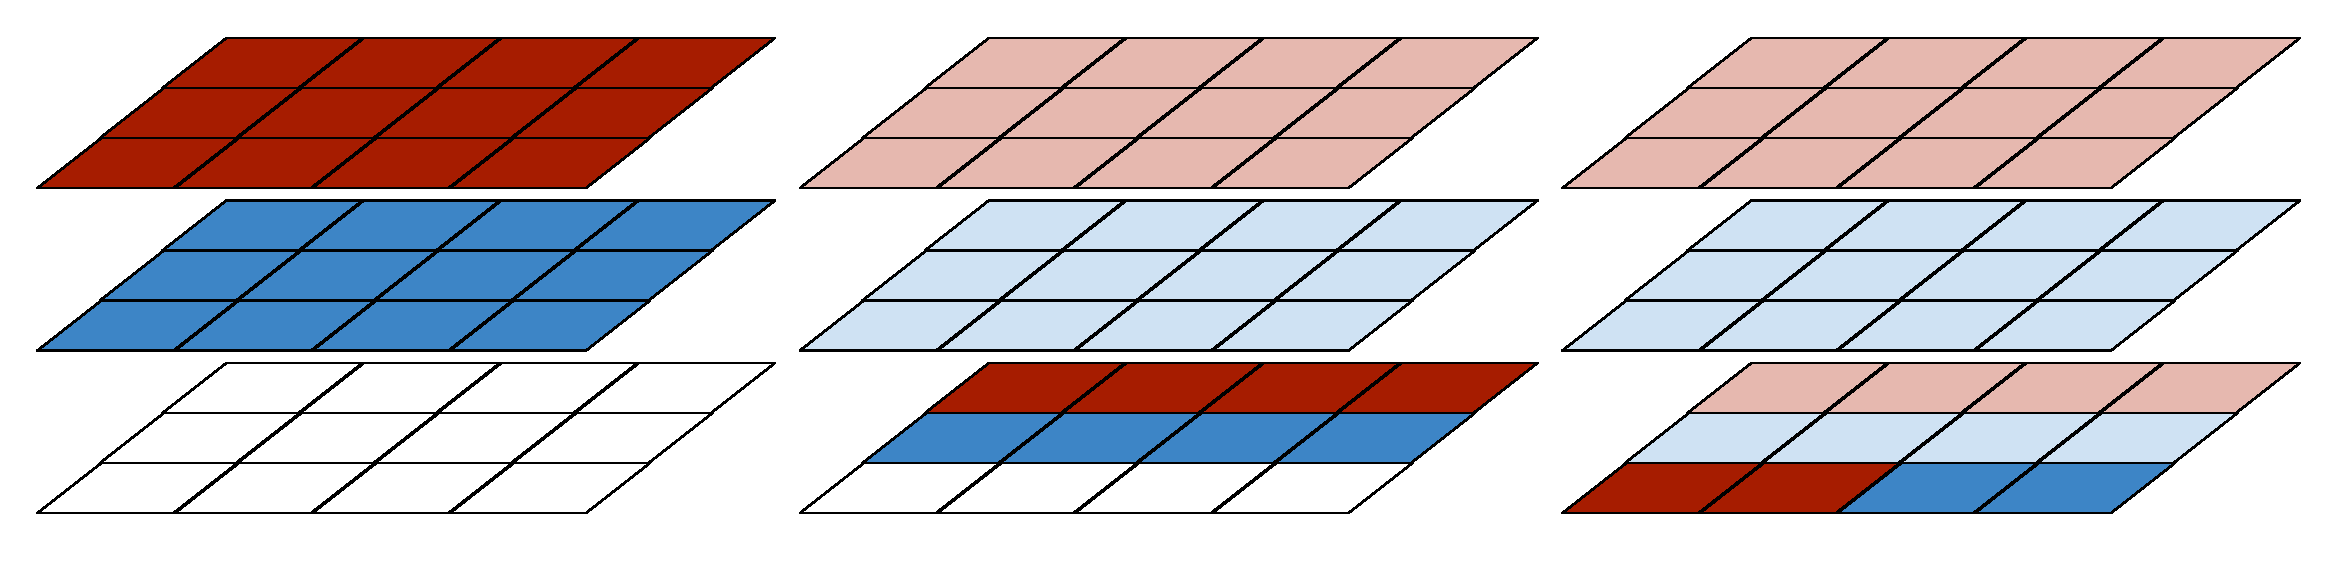
\includegraphics[width=0.97\linewidth]{fig/static2}
    \end{center}
    \caption{Computing the values of $F'=3$ channels of 2D images of
      size $4 \times 3$ using $T=2$ threads.  The three columns
      represent three stages.  The dark blue/red represent the values
      computed by the cores 1/2 during that stage.}
    \label{fig:problem-subdivision}
  \end{figure}

  An example of such sub--division is shown on
  Fig~\ref{fig:problem-subdivision}.  Note that each thread ends up
  computing the same amount of output voxels.  Furthermore, at each
  stage, each thread is solving the same \emph{Problem}, just with
  different data (SIMD).

  In each stage of the computation, each of the threads computes the
  values of the assigned sub--tensor in a serial fashion.  For that we
  need an efficient serial algorithm that can compute the values of an
  arbitrary sub--tensor.  It is improtatnt to first understand our
  serial algorithm, as it will introduce some restrictions on the
  problem sub--division.

  \subsection{Serial algorithm}

  Our serial algorithm computes $\mathcal{B} \le B$ sets of
  $\mathcal{F}' \le F'$ images each of size $\mathcal{D} \times
  \mathcal{H} \times \mathcal{W}$ ($\mathcal{D} \le D$, $\mathcal{H}
  \le H$, $\mathcal{W} \le W$).

  We take a divide and conquer approach to the serial algorithm.  We
  first divide the algorithm into primitives that performs $S^2$
  convolutions on $S$ input images, accumulating the result into $S$
  output images.  These primitives are further divided into
  sub--primitives that compute a small number of pixels of each of the
  $S$ output images.

  We first describe the most basic building block of our algorithm.
  The main goal of this primitive is to efficiently utilize the vector
  units as well as $L1$ cache.  We design the primitive so that it
  consists mainly of fused multiply--add instructions where two of the
  input arguments are stored in registers, and the third one is in
  $L1$ cache.  For the case of KNL, a single instructions can be used
  to perform such operation, whereas with AVX2 capable CPUs we need to
  use a set of auxiliary registers to first load the data from $L1$.
  We do not implement the two different cases, instead we let the
  compiler optimize the code for the specific architecture.

  The algorithm that computes a $S$ sub--images of size $\mathcal{D}
  \times \mathcal{H} \times \mathcal{W}$ is given
  on~\ref{alg:serial-forward-subtask}.  It consists of three main
  stages.  First, it loads the current values for the pixel values to
  the register file, then it performs a convolution with the
  corresponding kernels and input images, and finally stores the
  results back to memory.

  The convolution loop first goes over all kernel values, loading each
  of them into a register.  That value is then multiplied with the
  appropriate pixels from $S$ input images and accumulated to the
  registers containing the output set of pixels.

  The innermost loop over $S$ ensures efficient reuse of $L1$ cache.
  Mainly, it loops over $D \times H \times W$ pixels of $S$ images.
  As the L1 cache is larger than the number of registers times $S$, we
  expect that the consequent loops over $S$ will be guaranteed to have
  the value in L1 cache.

  This will however depend on the shape of $D \times H \times W$.  The
  main restriction of the shape is that it has to fit into the
  register file.  For the case of KNL we set the max size of elements
  to be 31 (as we need an extra register for the kernel values, and we
  have total of 32 registers).  For the case of AVX2, we set it to be
  at most 7.  This is because we need as many auxiliary registers to
  load input image pixels, as well as an extra for the kernel values
  (and we have 16 registers in total).

  We also prefer higher values for the least significant dimensions
  ($W$ in this case).  There are two main for this design choice
  which we discuss in sections.... They are hardware prefetching,
  cache associativity conflicts.

  The actual implementation of the primitive uses regular variables
  and it expect the compiler to assemble the code that uses the
  register file, as well as to optimally unroll the innermost loops.
  It turns out that both ICC and GCC produce the same optimal code as
  expected for AVX2, whereas only ICC produces optimal code for
  AVX512.  For AVX512, GCC fails to use the braadcast-fmadd
  instructions.

  We combined these, lowest level, primitives to compute $S^2$
  convolutions of $S$ input images by combining the primitives
  described above.  Each of the $S$ output images will be split into
  blocks of size at most $O_D \times O_H \times O_W$, and the
  computation will be performed by computing one block at the time.
  Note that not all the blocks will have the same size (in the case
  when the output image size is not divisible by the register blocking
  size).  By utilizing the C++'s template programming we will have a
  separate functions for computing blocks of different sizes.

  We prefer computing the blocks adjacent to the least significant
  dimension (in order to utilize the L2 cache and hardware prefetching
  \aleks{elaborate}.

  \subsection{Cache oblivious computation}


  \begin{figure}
    \begin{center}
      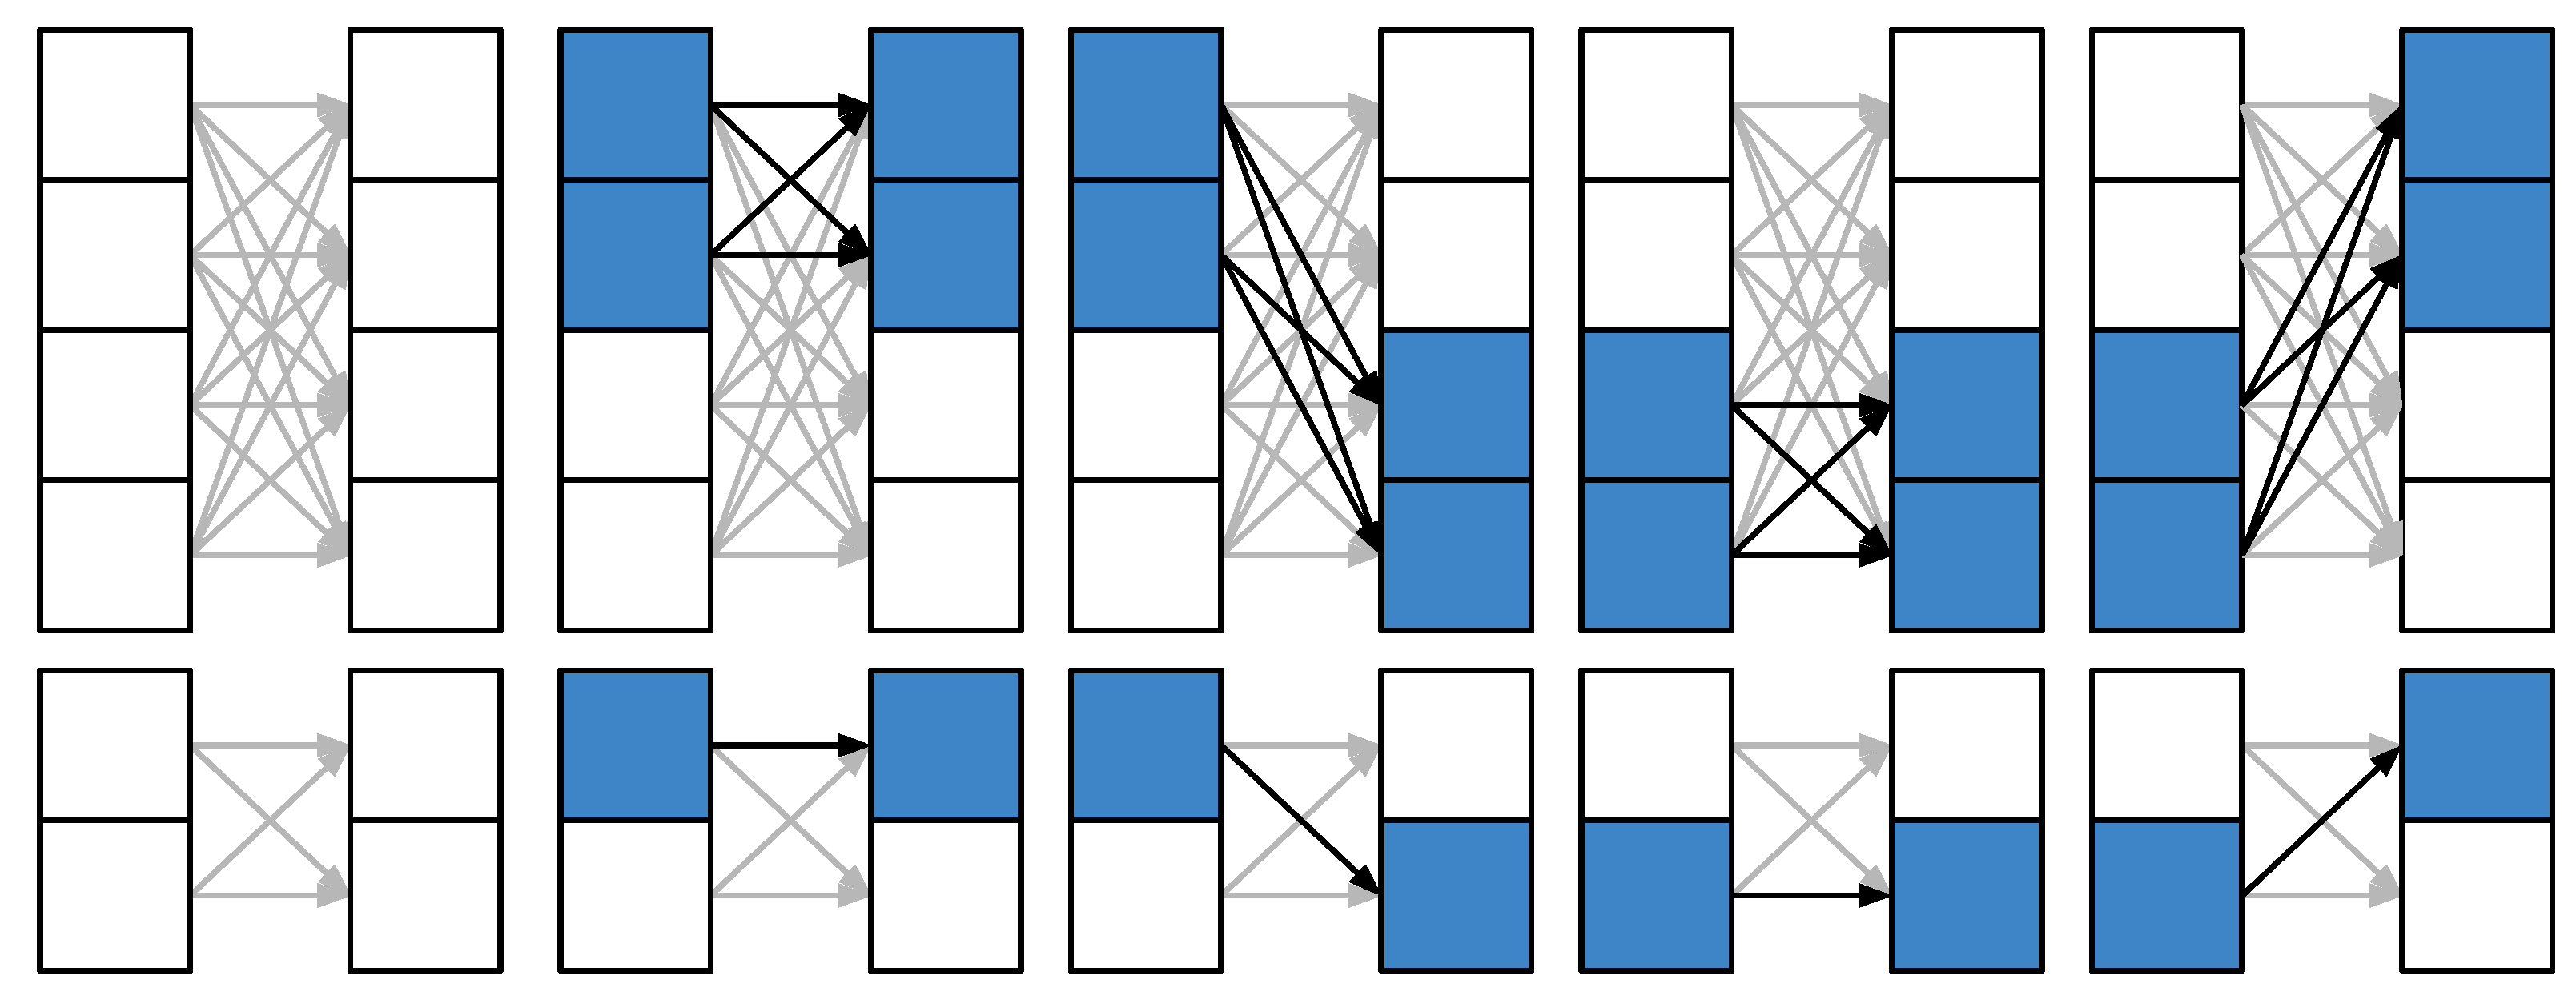
\includegraphics[width=0.8\linewidth]{fig/serialexec}
    \end{center}
    \caption{Cache oblivious compuitation.}
    \label{fig:full-exec}
  \end{figure}


  For each set of

  Given the primitive described above, we attempt to compute all $B
  \times \beta S \times D \times H \times W$ values in the following
  way.

  Given the primitives that perform the forward pass on $S$ input
  images and accumulate the result to $S$ output images, given $S^2$
  convolution kernels, we design a cache oblivious algorithm that
  performs the forward pass of an arbitrary number of input/output
  images.


  \subsection{Parallel execution}

  Our strategy for is relatively simple and is created during compile
  time.

  The main idea behind our static scheduling algorithm is to have all
  threads execute the same code, thus having the same number of
  operations/FLOPS to execute.

  To achieve this, we recursively divide the problem and assign a set
  of threads to execute a sub--problem.  To divide the problem among
  $T$ threads, we consider the smallest prime $P$ that divides $T$.
  We divide the problem into $P$ equal sub--problems, and recursively
  schedule the sub--problems to each of $T/P$ sub-threads.  If the
  problem can not be divided in exactly $P$ parts, we divide it into
  $P$ parts + a smaller remainder.  The remainder is then also
  recursively scheduled on all $T$ threads.

  All scheduling and code generation is done during compile--time with
  the magic of C++ templates.  Thus each sub--problem get's optimally
  compiled and optimized.

  The obvious advantage of such approach is that, by executing the
  exact same code, threads that share any level of cache, can leverage
  the caching of the instructions.  Other advantages are non--obvious,
  to understand them, we need to see how the problem gets recursively
  divided.  For simplicity, we will assume that the number of
  available threads is a power of $2$, the same approach can be taken
  for an arbitrary number of available threads.  However, in practice,
  best divisions can be obtained if $T$ is a product of small primes.
  Our implementation limits $T$ to be product of $2,3,5$ and $7$.


  \subsection{Serial algorithm}

  In this section we describe both the serial vectorized approach to
  computing the forward and backward pass as well as a parallel
  algorithm that combines these serial primitives.

  As described before, we keep two copies of the kernels in two
  different memory layouts, one suitable for both the forward and
  backward pass computation.  Our algorithm is supports implicit zero
  padding, hence both the forward and backward pass can be computed
  using the same algorithm.

  \subsection{Cache, etc...}

  In order to be portable, our algorithm doesn't assume any specific
  size of available caches.  However it assumes that small $L1$ data
  cache is present, able to fit $2 \times S \times R$ floats.  $R$
  represents the number of available SIMD registers.  This is true for
  all commercially available CPUs.

  Also, we assume presence of higher levels of cache (L2,L3), however,
  our algorithm is oblivious to the size of the cache.  Having more
  cache will, however improve the performances of the algorithm.
